\section{Experimental Plan}
\label{sec:experimentalPlan}
\todo[inline]{Plan for experimental research. Include experiments and series of experiments planned.}
\todo[inline]{Planned experiments and what questions the experiements aim to answer. Connected to research questions}
\begin{itemize}
\item Comparison baseline model and curriculum model
\item Comparison crossentropy and bootstrapping for several
levels of label degradation. 
\item Test curriculum for different dataset sizes. Will advantage of curriculum disappear for larger datasets?
\item Larger dataset for bootstrapping?
\item Can curriculum learning combined with bootstrapping loss function further improve results for label noise?
\item How much does the competence of the curriculum teacher affect the results of curriculum learning?
\end{itemize}

\begin{figure}
\begin{center}
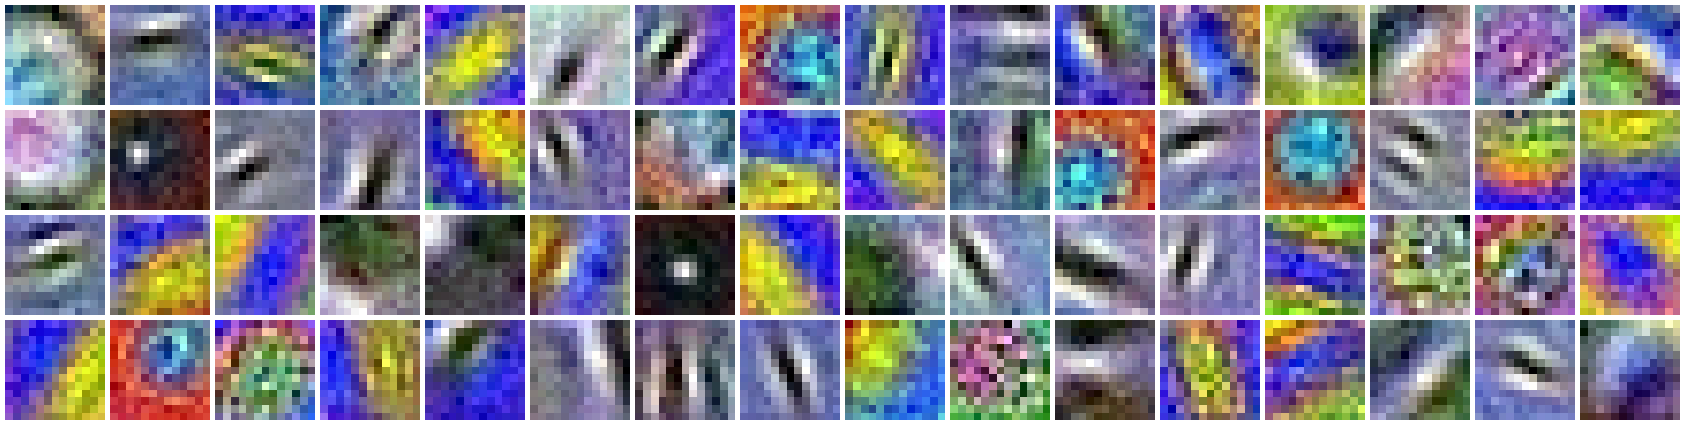
\includegraphics[width=1\columnwidth]{figs/network/Filter_unblurred.png}
\caption[Visualization of filter map]{Visualization of filter maps from the first convolutional layer of a trained network.}
\label{fig:convoluional_first_layer_visualization}
\end{center}
\end{figure}

\begin{table}[htp]
\caption{Planned experiments}
\begin{center}
\begin{adjustbox}{max width=\textwidth}
\begin{tabular}{+l ^l ^l ^p{5cm}}\hline
\rowstyle{\bfseries}
  ID & RQ & Dataset & Description\\\hline
  E1 & RQ2 & Norwegian Roads Dataset Vbase & Performance of curriculum learning at different thresholds $D_\theta$. \\
  E2 & RQ2 & Massachusetts Roads Dataset & Curriculum, baseline and anti-curriculum comparison. \\
  E3 & RQ1 & Massachusetts Roads Dataset & Bootstrapping versus baseline at different levels of label noise \\
  E4 & RQ1 & Norwegian Roads Dataset N50/Vbase & Performance of bootstrapping for dataset with a lot of label noise \\\hline
\end{tabular}
\end{adjustbox}
\end{center}
\label{tab:planned_experiments}
\end{table}
